\documentclass{beamer}
\usetheme{default}
\usepackage{subfig}

\title{Work of the Past, Work of the Future}
\author{David H. Autor}



\begin{document}
	
\begin{frame}

    \maketitle
    
\end{frame}

\begin{frame}{Introduction}

\begin{itemize}
	
	\item Since the 1980's the average U.S. worker has become more educated and technologically equipped.
	
	\begin{itemize}
		
		\item The skillset gained from educational attainment and technological prowess are concentrated among the high-skill occupations.
		
		\begin{itemize}
			
			\item Productivty gains over the past 3-4 decades have come from these high-skill occupations.
			
		\end{itemize}
		
	\end{itemize}

	\bigskip
	
	\item High, medium, and low-skill workers work side-by-side in a work enviromnent so productivity gains should be shared to some degree.
	
	\begin{itemize}
		
		\item Can be thought as capital deepening without loss of generality.
		
		\item We then expect real wages to rise for workers in low and high-skill occupations.
		
	\end{itemize}
	
\end{itemize}

\end{frame}

\begin{frame}{Summary of Results}

\begin{itemize}
	
	\item Non-college workers in middle-skill jobs (admin., clerical, production) have been forced into traditionally low-skill occupations.
	
	\bigskip
	
	\item Encroachment of occupational polarization may (in part explain) the fall in real wages of non-college workers over the last three decades.
	\begin{itemize}
		\item There is an important geographical component to this!
	\end{itemize}

	\bigskip
	
	\item Overall, the urban wage premium for non-college workers has disappeared. Dense cities are only alluring for college educated.
	\begin{itemize}
		\item Autor says less migration will raise non-college wages.
		\item Aging population in suburbs provides job creation for non-college workers.
	\end{itemize}

	
\end{itemize}

\end{frame}


\begin{frame}{Real Wages from 1963-2017}

\begin{figure}
	\begin{center}
		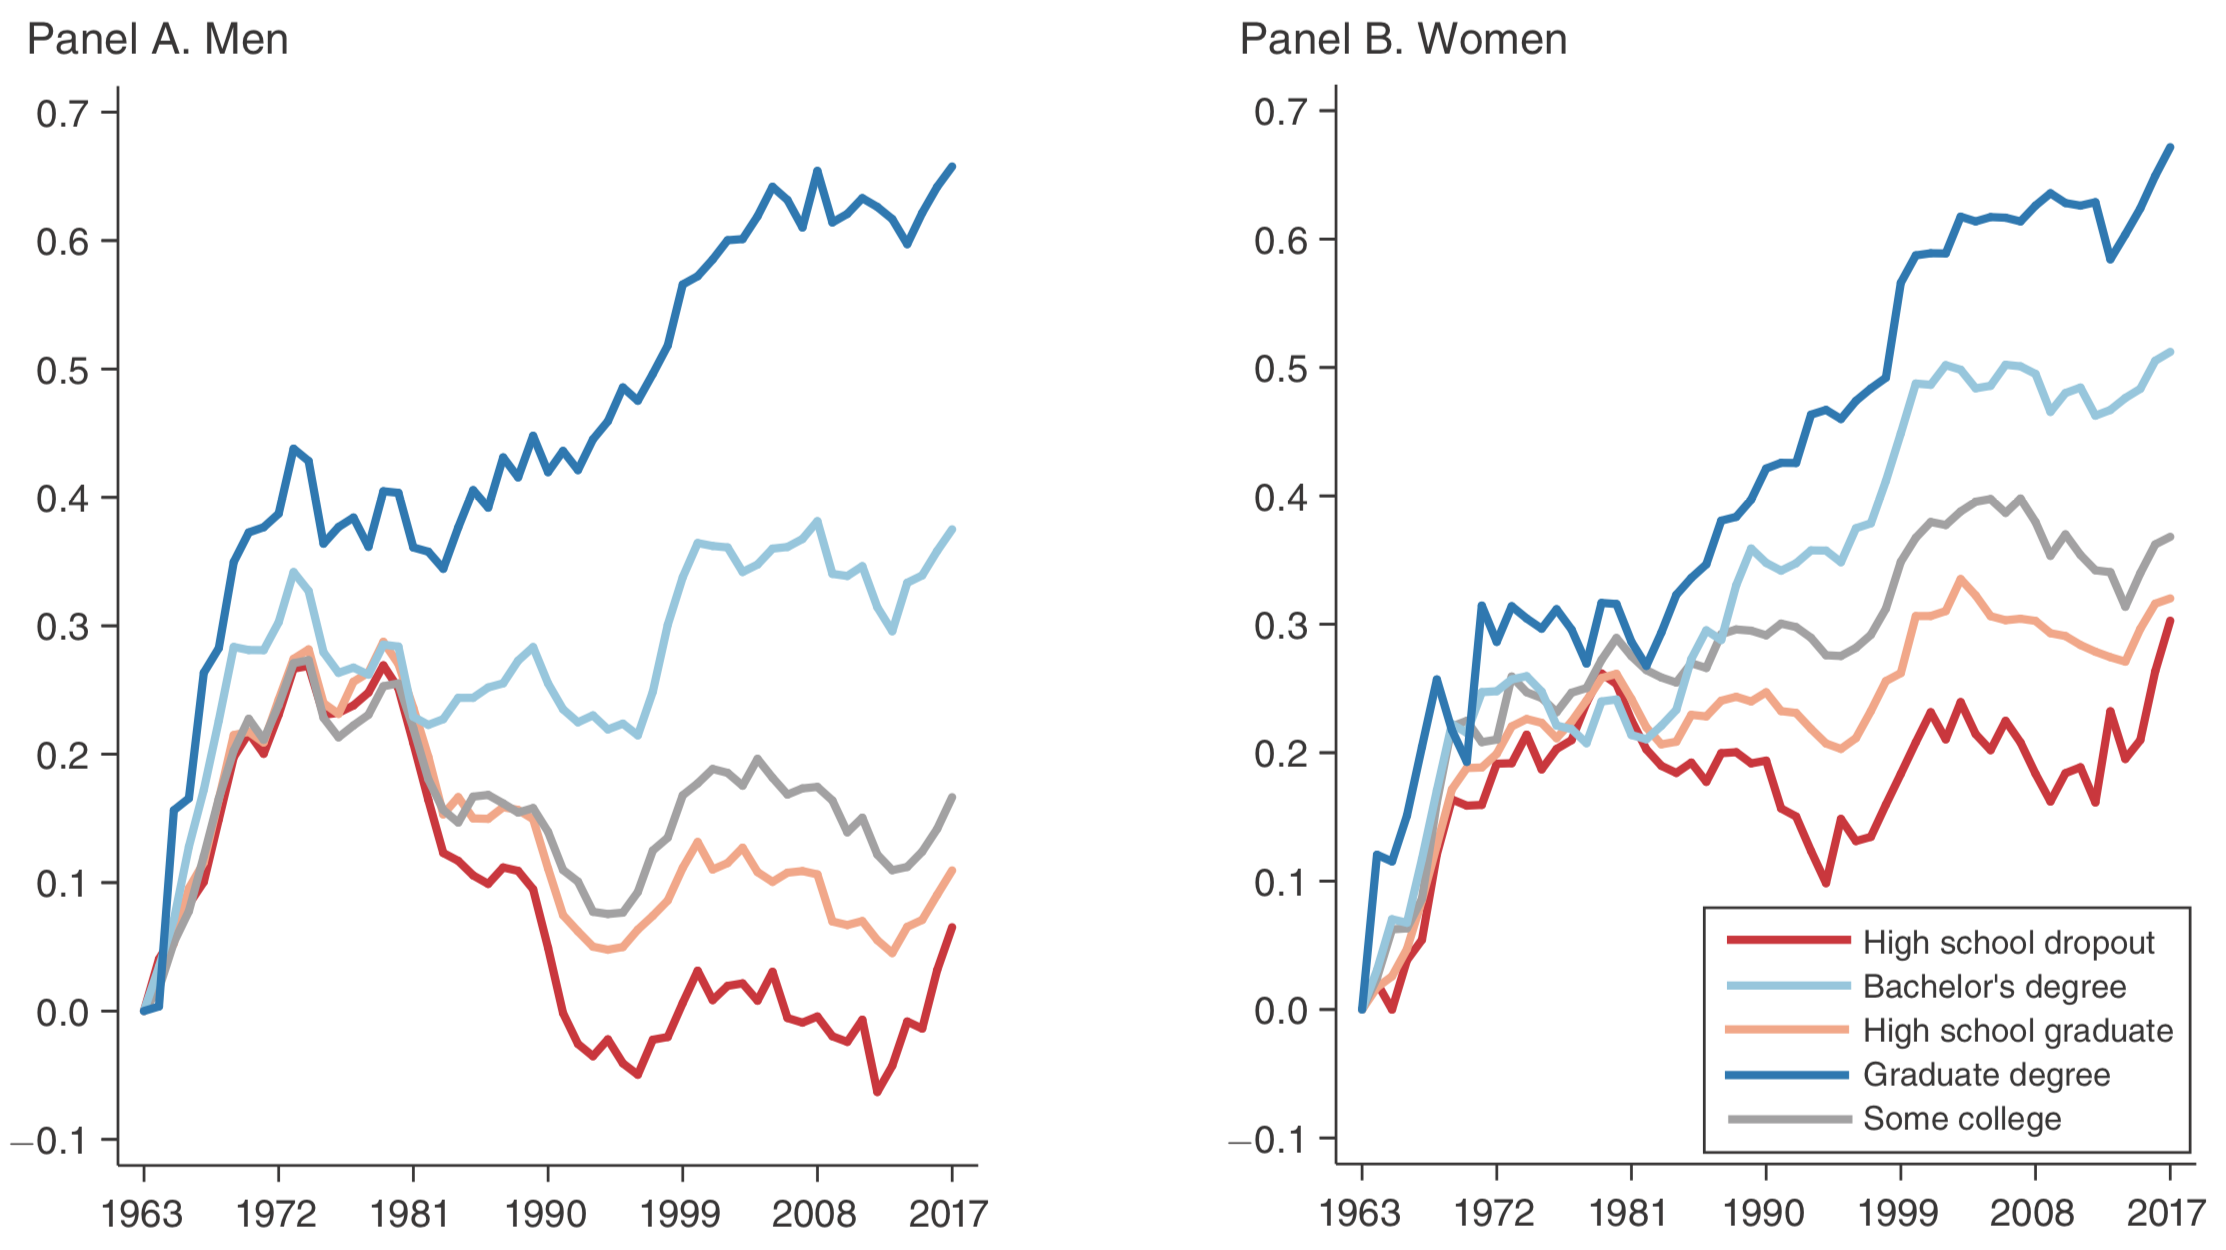
\includegraphics[scale=0.25]{Figures/Fig1_RealWages}
		\caption{Cumulative Change in Real Weekly Earnings of Working-Age Adults Ages 18-64, 1963-2017}
	\end{center}

\end{figure}

\end{frame}


\begin{frame}{Interpreting Change in Real Wages}

\begin{itemize}
	
	\item Robust real wage growth for all education groups and genders from '63 to 72'.
	
	\item Real wages stagnate from '73 (first U.S. oil shock) to '79 across distribution of workers.
	
	\item Rising wage inequality from 1980 forward.
	\begin{itemize}
		\item Well documented that productivity gains among high-skill ofset supply effects.
		\item Real wages particularly fall sharply men with less than a bachelor's degree.
	\end{itemize}

	\item If high and low-skill workers are gross complements (elasticity of substitution in production is greater than one) than low-skill worker wages should have risen as well.

	
	
	
\end{itemize}

\end{frame}



\begin{frame}{Occupational Polarization}

\begin{itemize}
	
	\item Foundational assumption of the skill demand literature (Tinbergen, 1974): technological progress complements—and hence raises demand for educated workers
	
	\begin{itemize}
		
		\item Hence, highly educated worker should see their work change.
		
		\item Is this what we observe in the world?
		
	\end{itemize} 

	\bigskip
	
	\item Descriptive analysis of changes in employments shares (by skill and education) show technology has affected low skill workers the most
	
	\begin{itemize}
		
		\item From 1980 to 2016, non-college, middle-skill employment fell by 14 percentage points.
		
		\item 87\% of the decline is explained by the movement of those workers into traditionally low-skill work.
		
		
	\end{itemize}

	\bigskip

	\item Technological change has been deskilling for non-college workers, forcing them into low-skill, low-wage jobs.
	
\end{itemize}

\end{frame}


\begin{frame}{Occupational Change from 1980-2016}

\begin{figure}
	\begin{center}
		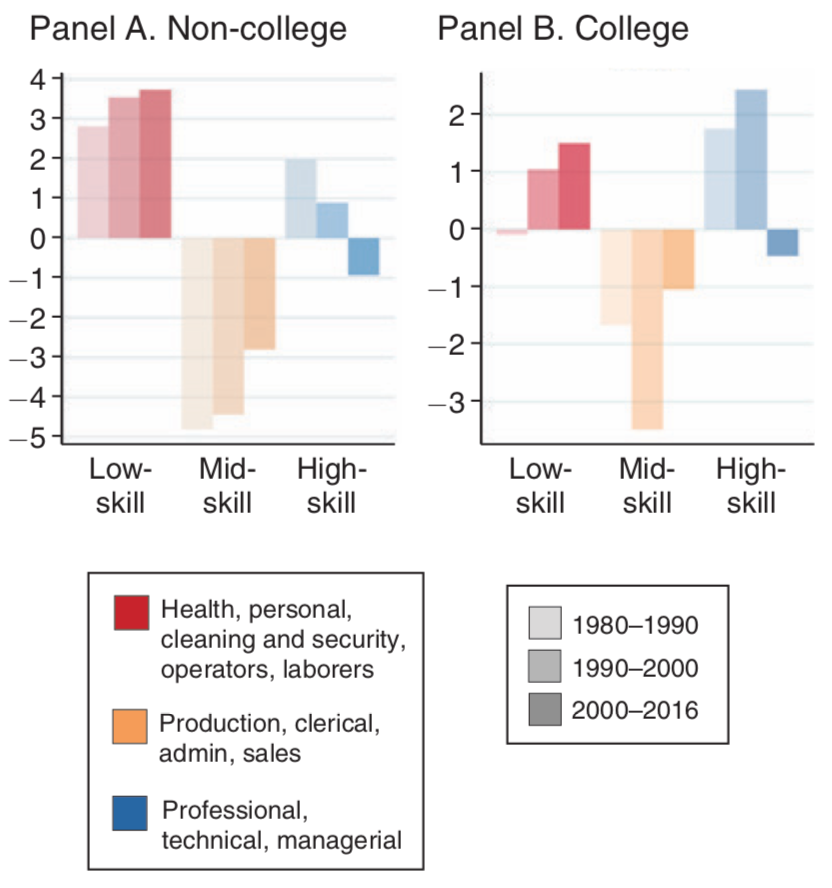
\includegraphics[scale=0.35]{Figures/Fig2_OccChange}
		\caption{Change in occupational employment share among working-age adults, from 1980-2016; \newline \tiny{\textbf{low-skill}: services, transportation, laborer, and construction workers; \newline \textbf{mid-skill}: clerical, administrative support, sales, and production workers; \newline \textbf{high-skill}: professional, technical, and managerial workers.}}
	\end{center}
	
\end{figure}

\end{frame}


\begin{frame}{Can Occupational Changes Explain Wage Divergence}

\begin{itemize}
	
	
	\item Partial equilibrium calculation to construct counterfactual wages
	
	\begin{itemize}
		
		\item Hold the occupational wage structure fixed at its 1978 level
		
		\item Allow distribution of workers by education and gender to shift across occupations 
		
	\end{itemize} 

	\medskip

	\item Let $j$ denote education group and $k$ denote occupation between years $t_0$ and $t_1$. 
	

	\begin{equation*}
		\Delta \bar{w}_{j\tau} = \sum_k \Big( \alpha_{jkt_1}\omega_{jkt_1} - \alpha_{jkt_0}\omega_{jkt_0} \Big)
	\end{equation*},
	
	 %where $\alpha_{jkt}$ is the fraction of group j workers in occupation k at time t, and and \omega_{jkt} is their mean log wage in that occupation and year
	 
	 \item Isolate $\alpha$ while holding $\omega$ fixed.
	 
	 \begin{equation}
	 	\Delta \tilde{w}_{j\tau} = \sum_k \bar{w}_{jkt_0} \Big( \alpha_{jkt_1} - \alpha_{jkt_0} \Big)
	 \end{equation}
	 
\end{itemize}

\end{frame}


\begin{frame}{Partial Equilibrium Effect of Occupational Change}

\begin{figure}
	\begin{center}
		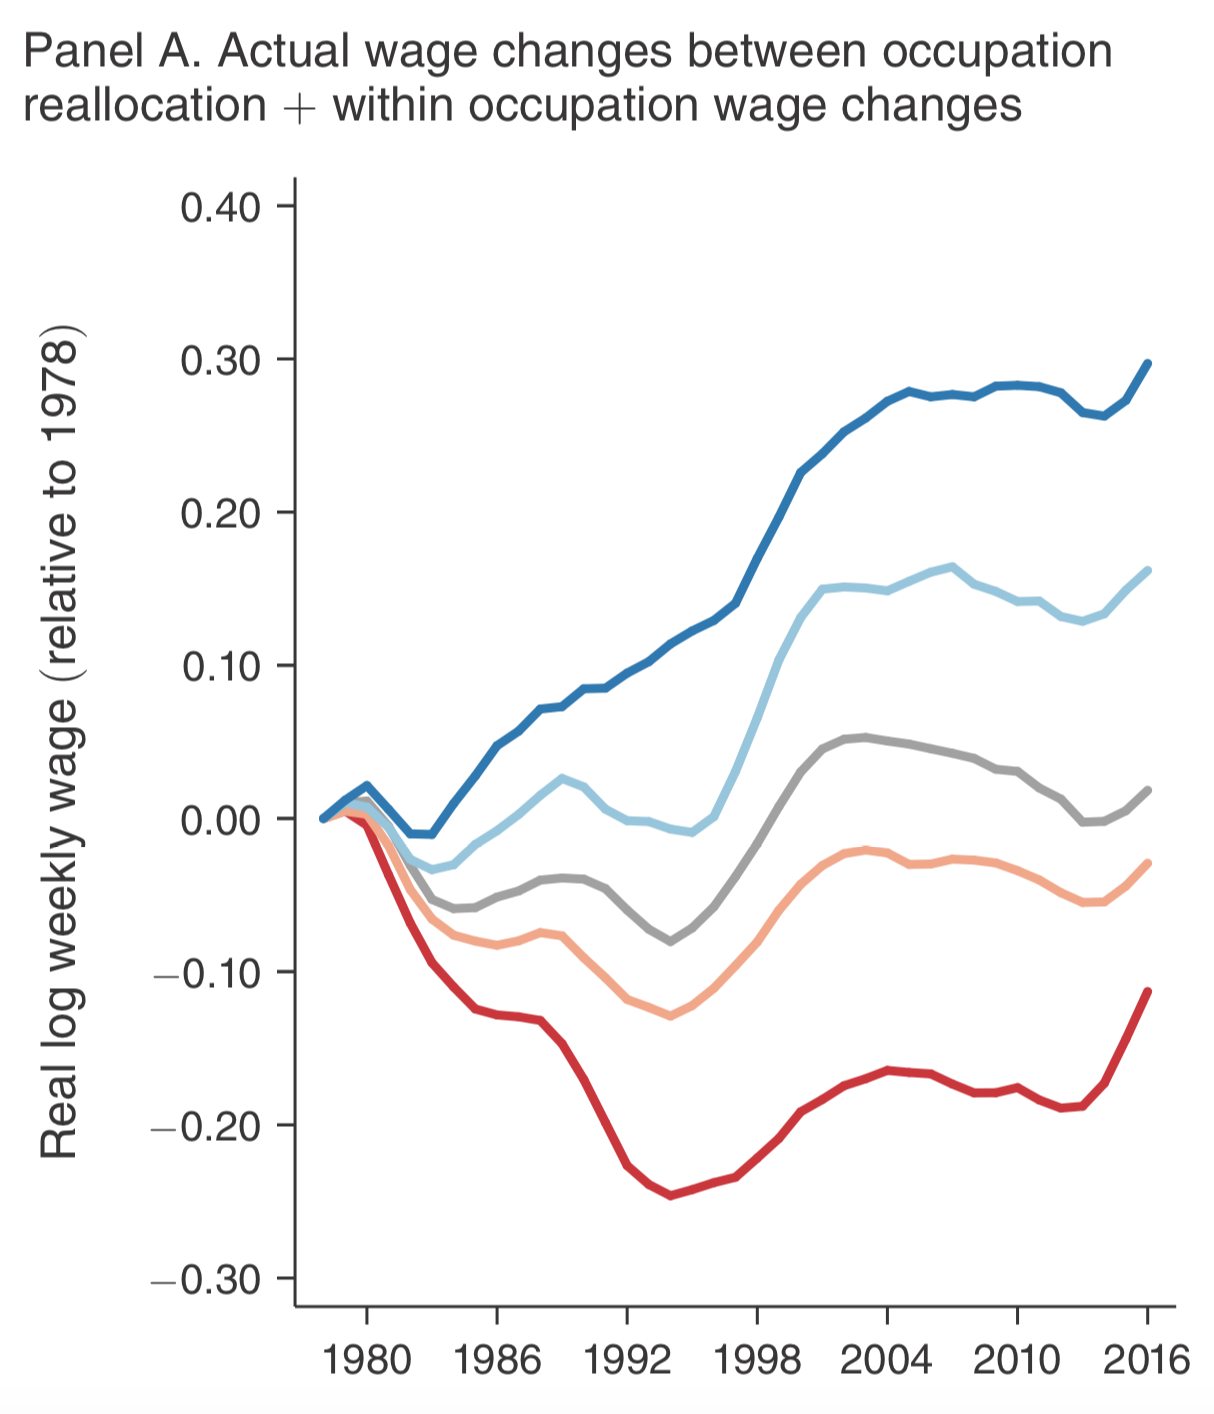
\includegraphics[scale=0.2]{Figures/Fig3A_ActualWageChange}
		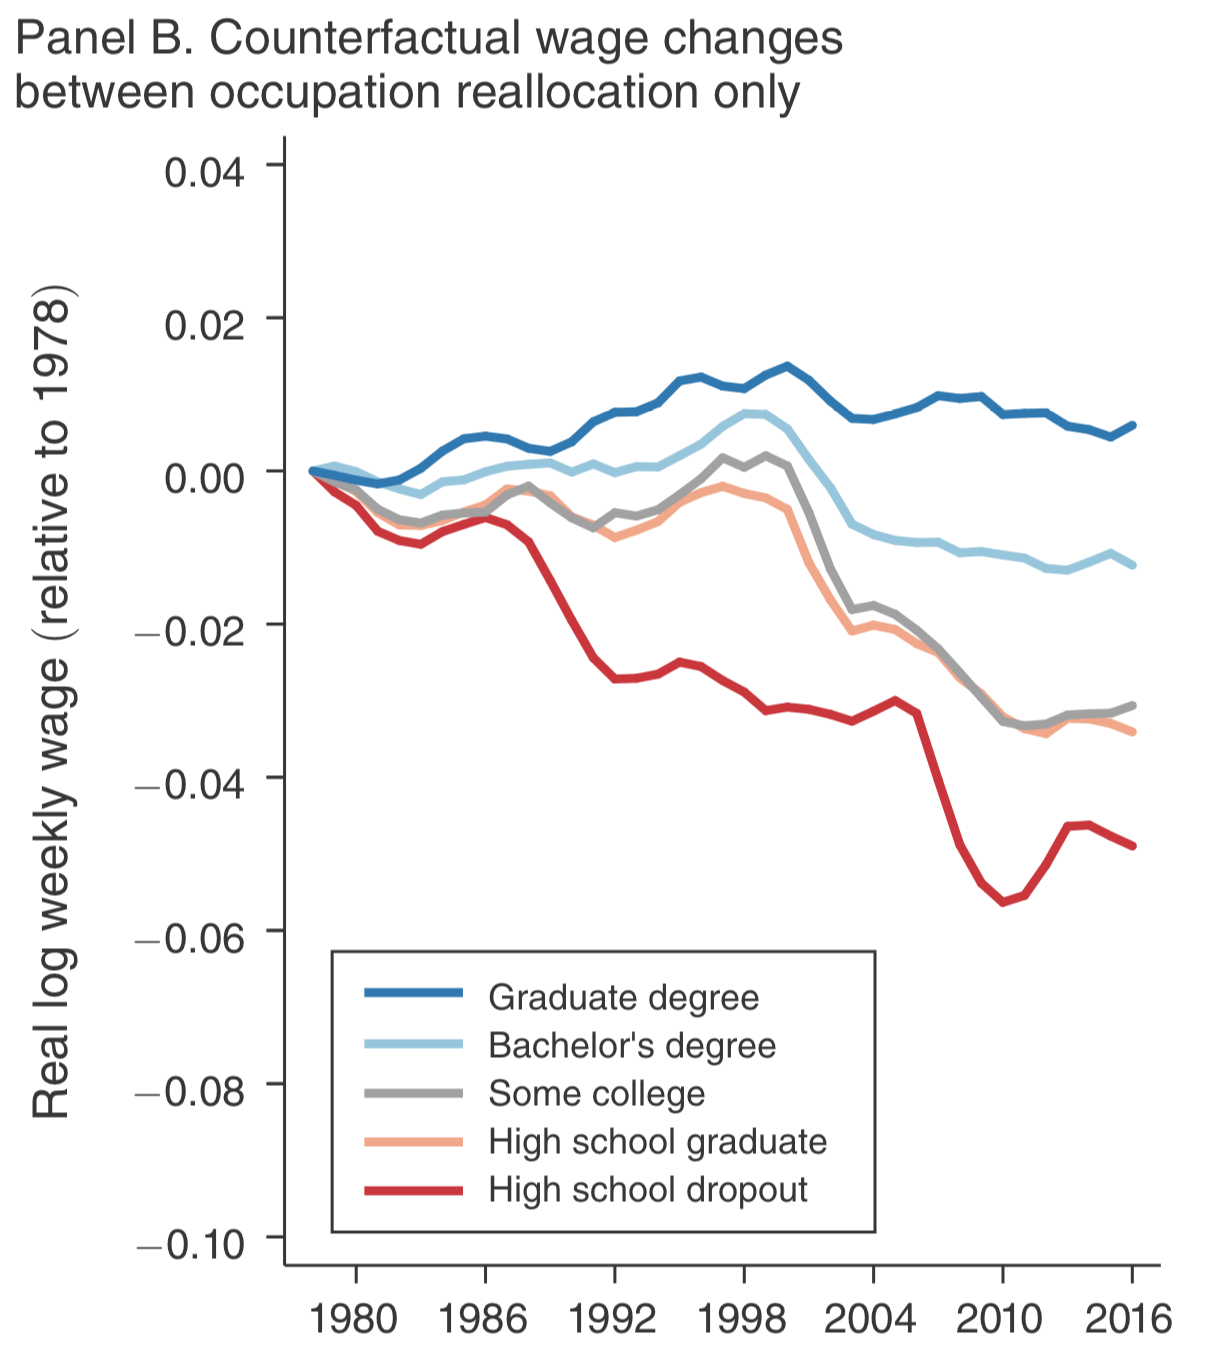
\includegraphics[scale=0.2]{Figures/Fig3B_CounterfactualWageChange}
		\caption{Real log wage growth by education group 1978 to 2016: 1978 to 2016: Observed versus Between Occupation Reallocation Component, 1970–2016}
	\end{center}
	
\end{figure}

\end{frame}


\begin{frame}{Problems with Partial Equilibrium}

	\begin{enumerate}
		
		\item Miss the strong upward trend in college-educated real wages
		
		\begin{itemize}
			
			\item real wages fixed at their 1978 levels, so series omits wage-augmenting productivity growth
			
		\end{itemize}
	
			\item Magnitude of change is way off (less than 5 times what we observe)
	
	\begin{itemize}
		
		\item Assuption that the decline of middle-skill occupations has occurred at the average (log) wage level within each occupation-education-gender group.
		
		\item Violated if the marginal declining (or growing) job within an occupation differed from the average of that occupation.
		
	\end{itemize}

		
	\end{enumerate}

	\begin{itemize}
		
		\item Violation: the decline of middle-wage occupations were particularly concentrated in cities and metro areas where wage levels are consistently higher.
		
	\end{itemize}

\end{frame}


\begin{frame}{The Geography of Polarization}

\begin{itemize}
	
	\item High-skill occupations and industries tend to be concentrated in high-density cities with highly educated populations.
	
	\bigskip
	
	\item Autor examines relationship between population density and occupational structure at commuting zone level between 1970 and 2015.
	
	\item For consistency, plot log population density in 1970 against binned employment share (weighted by population in each CZ).
	
	\begin{itemize}
		
		\item Roughly 5\% of population represented by each bin.
		
	\end{itemize}

	\bigskip

	\item Autor finds no change in relationship for low-skill occ., gradual inversion for middle-skill occ., and level shifts for high-skill occ.
	
\end{itemize}

\end{frame}


\begin{frame}{Geographic Concentrations of Occupations by Skill-Level}

\begin{figure}
	\begin{center}
		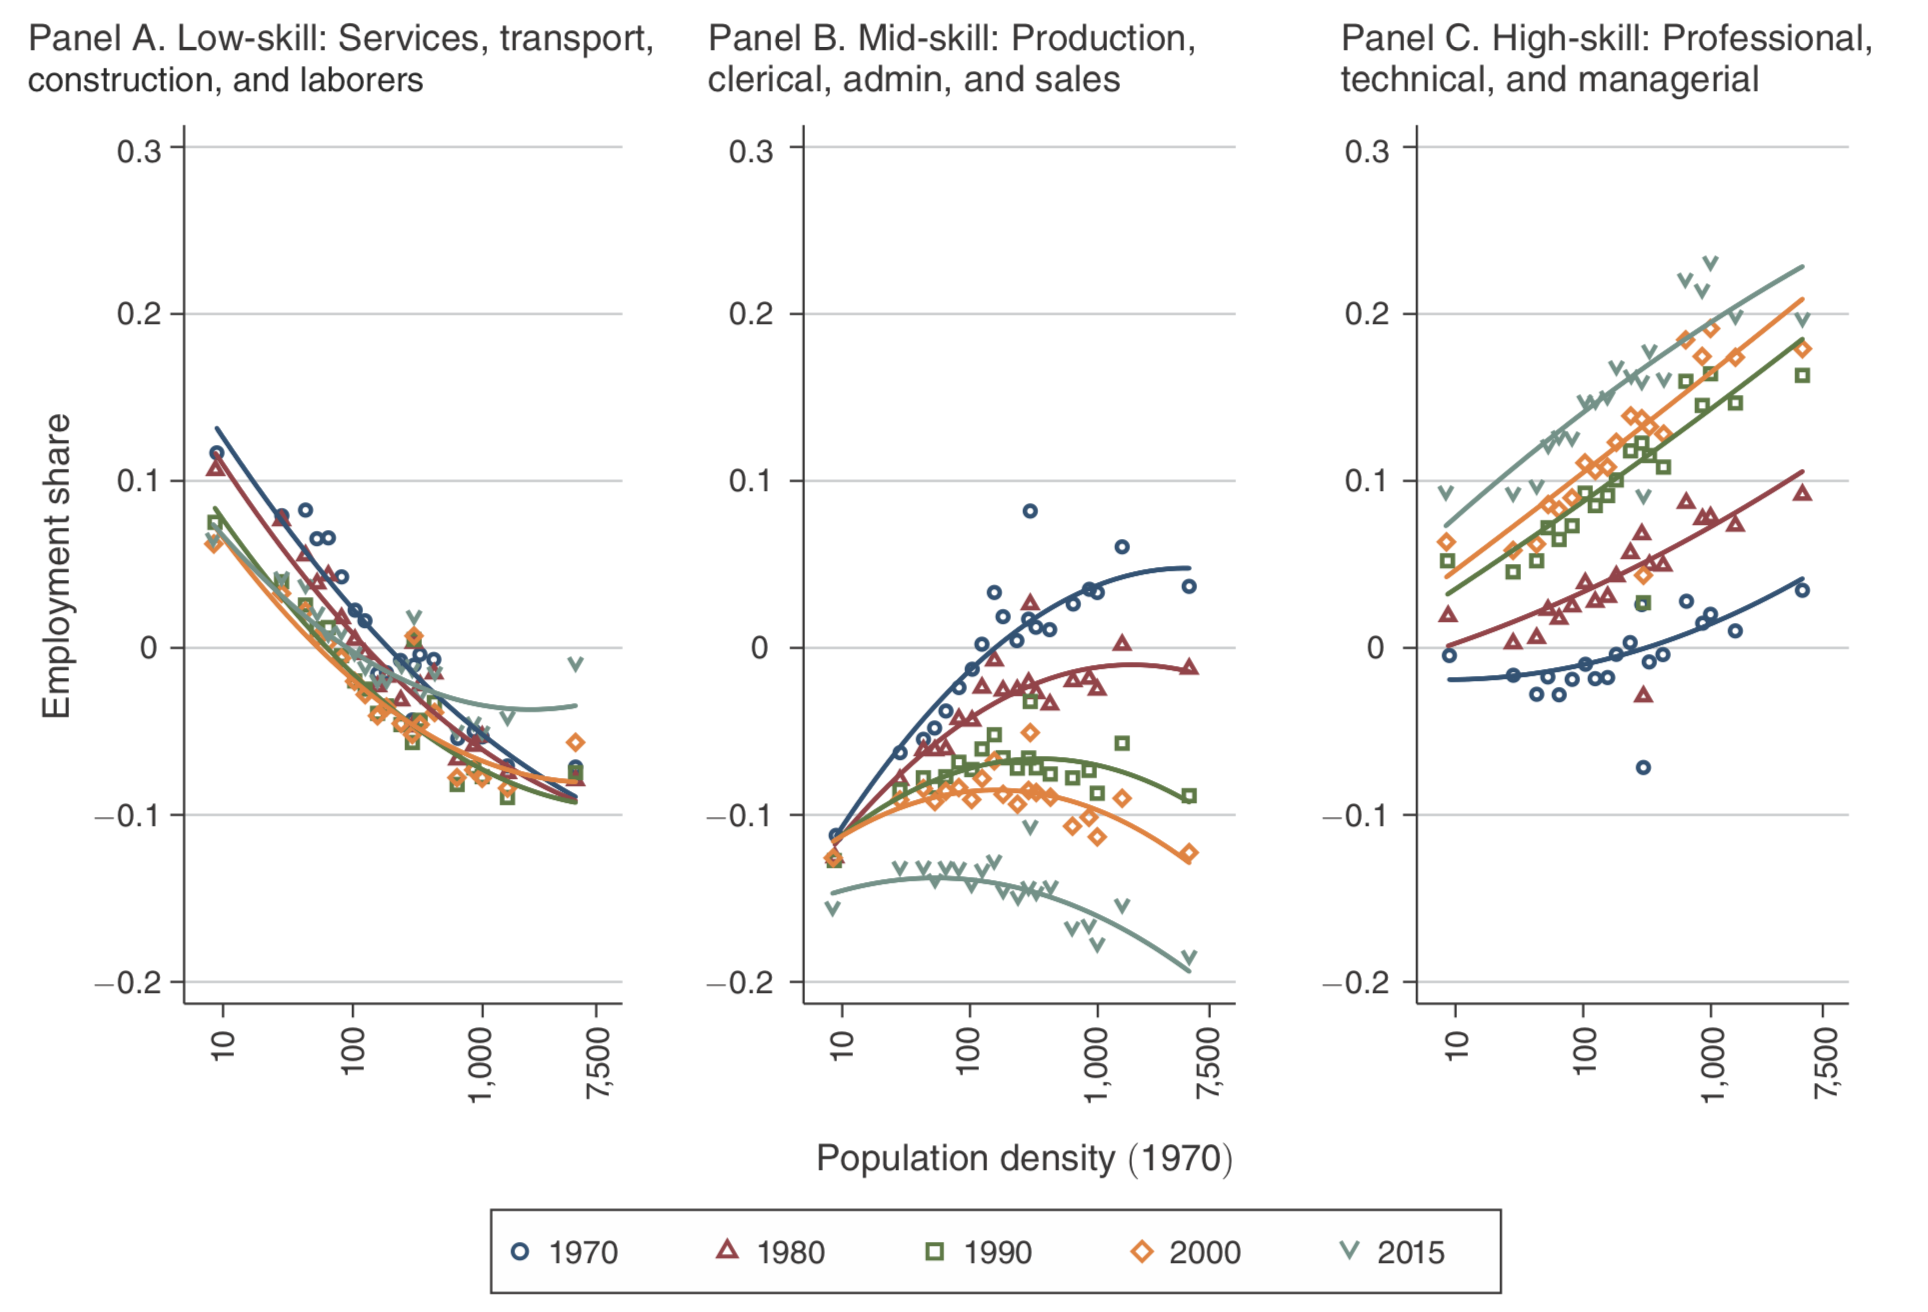
\includegraphics[scale=0.29]{Figures/Fig4_OccShares_LogDensity}

		\caption{Occupational Employment Shares among Working-Age Adults by Commuting Zone Population Density, 1970–2015: Level Relative to 1970 Mean}
	\end{center}
	
\end{figure}


\end{frame}


\begin{frame}{Geographic Concentrations of Occupations by Skill-Level and Education (college)}

\begin{figure}
	\begin{center}
		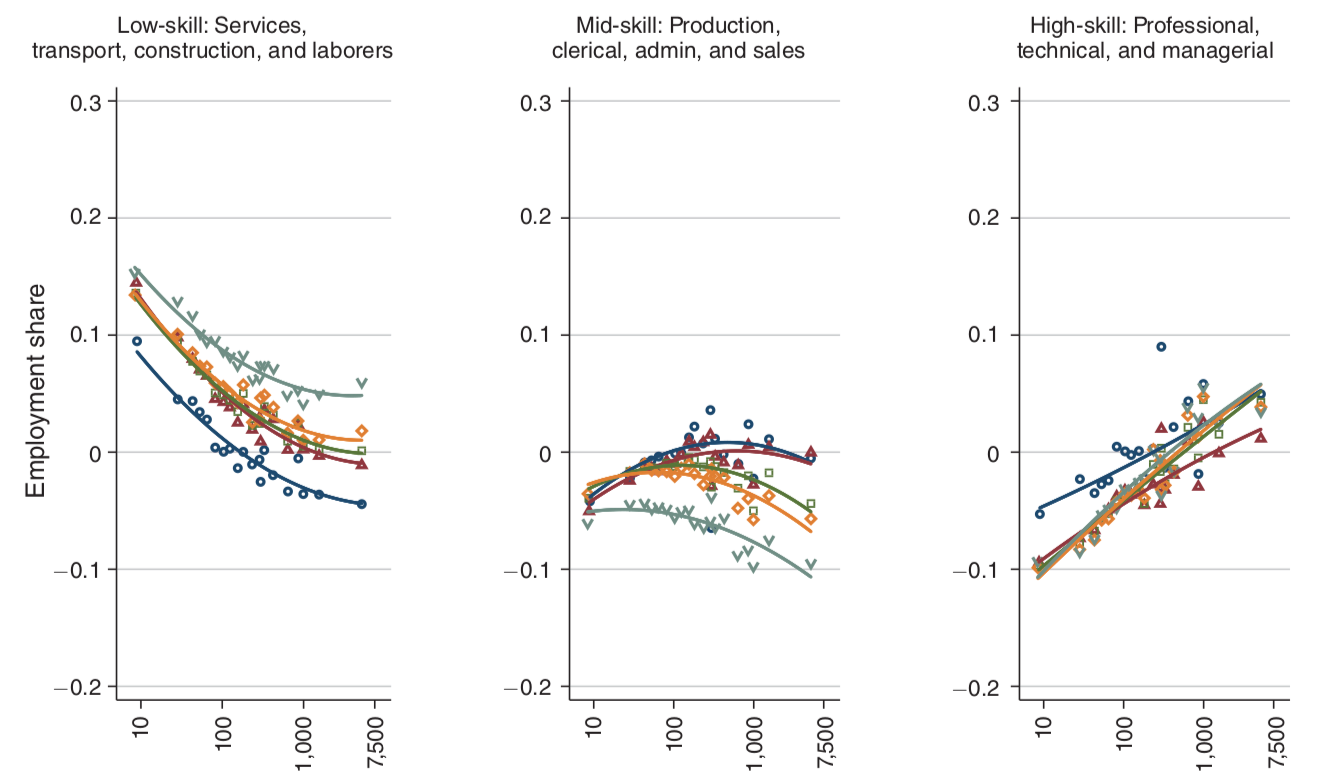
\includegraphics[scale=0.4]{Figures/Fig5A_OccShare_Education} 
		\caption{Occupational employment shares among college adults by commuting zone population density, 1970-2015: level relative to 1970 mean}
	\end{center}
	
\end{figure}

\end{frame}


\begin{frame}{Geographic Concentrations of Occupations by Skill-Level and Education (non-college)}

\begin{figure}
	\begin{center}
		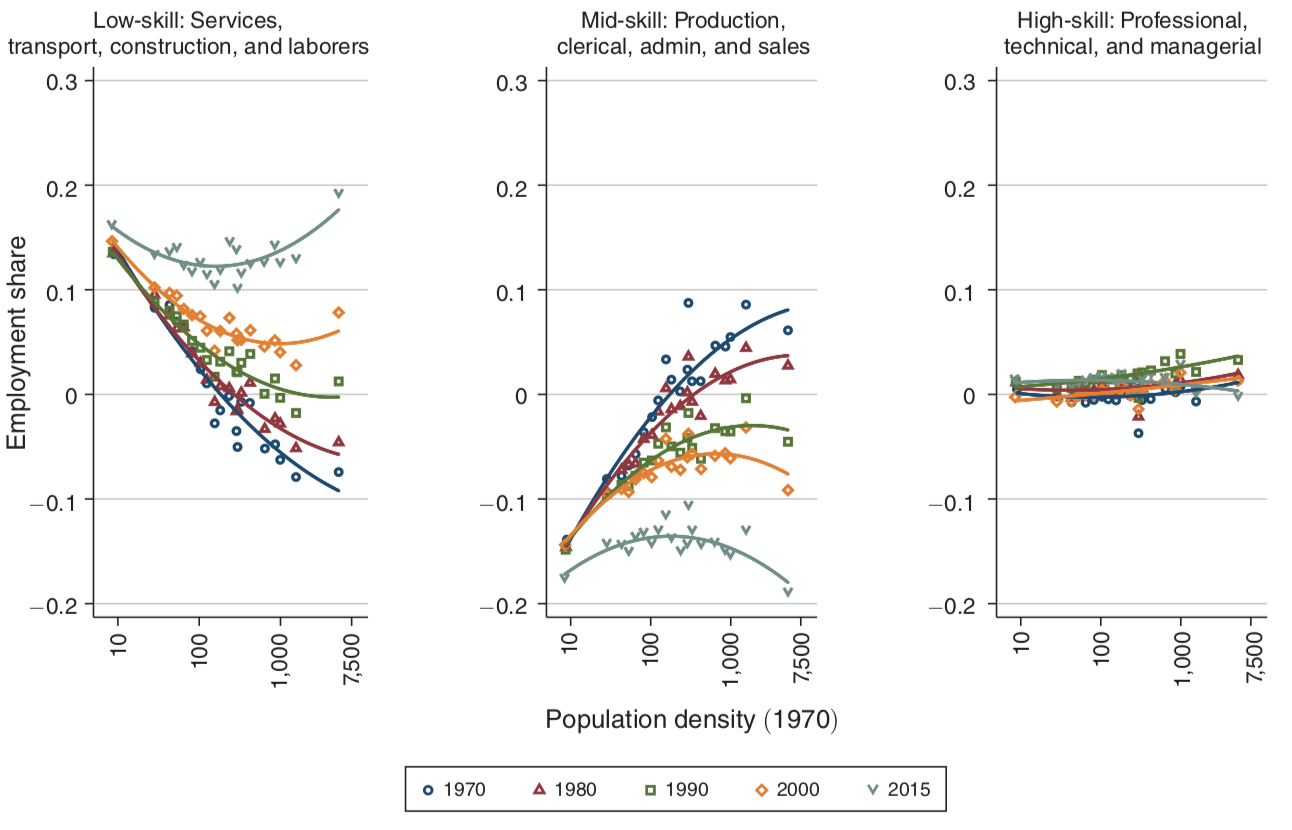
\includegraphics[scale=0.4]{Figures/Fig5B_OccShare_Education}
		\caption{Occupational employment shares among non-college adults by commuting zone population density, 1970-2015: level relative to 1970 mean}
	\end{center}
	
\end{figure}

\end{frame}


\begin{frame}{Interpreting Changing Geographic Concentrations of Occupations}

\begin{itemize}
	
	\item In 1970, non-college workers in the densest CZs were approximately 25 percentage points more likely to work in middle-skill occupations.
	\begin{itemize}
		\item The opposite is true today.
	\end{itemize}
	
	\bigskip
	
	\item Decline of middle-skill occupations has meant a profound reallocation of non-college workers in large cities from middle-skill production to low-skill, low-wage jobs.
	
	\bigskip
	
	\item Possibile that the shifting density gradient in occ. structure from the increasingly bimodal educational and nativity structure of denser CZs.
	\begin{itemize}
		\item Discussed in paper/lecture, but I won't talk about it.
	\end{itemize}
	
	
\end{itemize}

\end{frame}

\begin{frame}{Where were/are the Middle-skill Jobs?}

\begin{figure}
	\begin{center}
		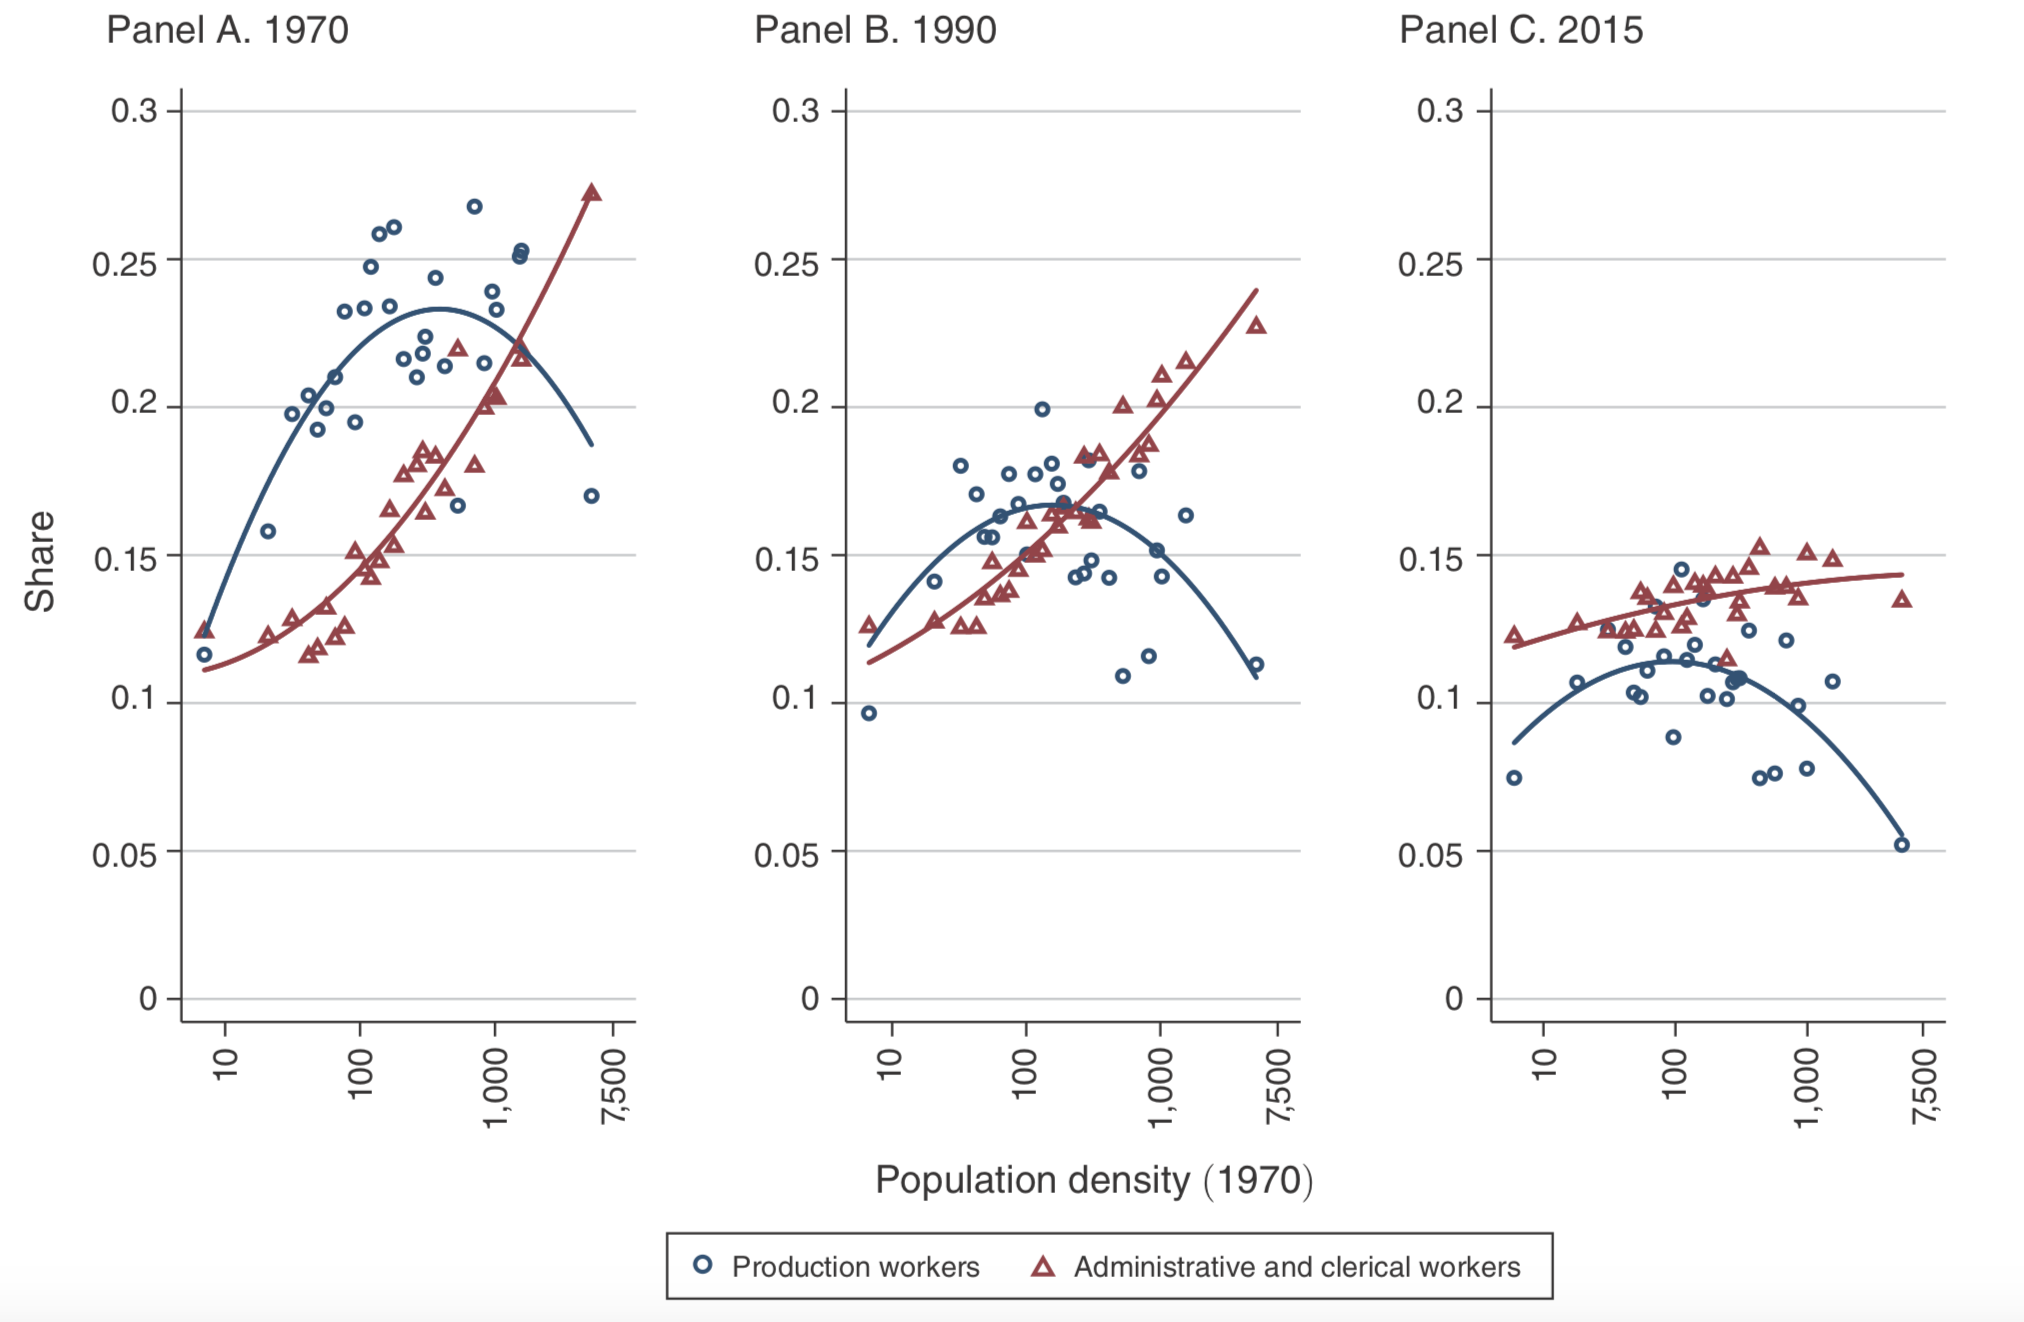
\includegraphics[scale=0.24]{Figures/Fig6_MidSkill_EmpSh}
		\caption{Production and Administrative and Clerical Employment Shares among Non-College Adults, 1970-2015}
	\end{center}
\end{figure}

\begin{itemize}
	
	\item Reversal of opportunity for better pay in urban areas for non-college workers
	
\end{itemize}

\end{frame}

\begin{frame}{Non-college Urban Wage Premium}

\begin{itemize}

\item Urban wage premium (widely documented) often explained by knowlegdge spillovers from college-education workers.

\begin{itemize}
	
	\item In urban areas, non-college worker are colocated alongside the highly-educated knowledge workers
	\item Possible source for positive occupational and wage density gradient for non-college workers.
	
\end{itemize}

\item Autor finds that urban wage-premium has in fact declined for non-college.

\item Could be from shifting occ. structure of market, but could also be:
\begin{enumerate}
	
	\item Shifting age structure of across density gradient.
	
	\item Shifting educational structure of "non-college".
	
	\item Lingering after-effects of the Great Recession.
	
\end{enumerate}

\end{itemize}

\end{frame}


\begin{frame}{Unfiltered Urban Wage Premium}

\begin{figure}
	\begin{center}
		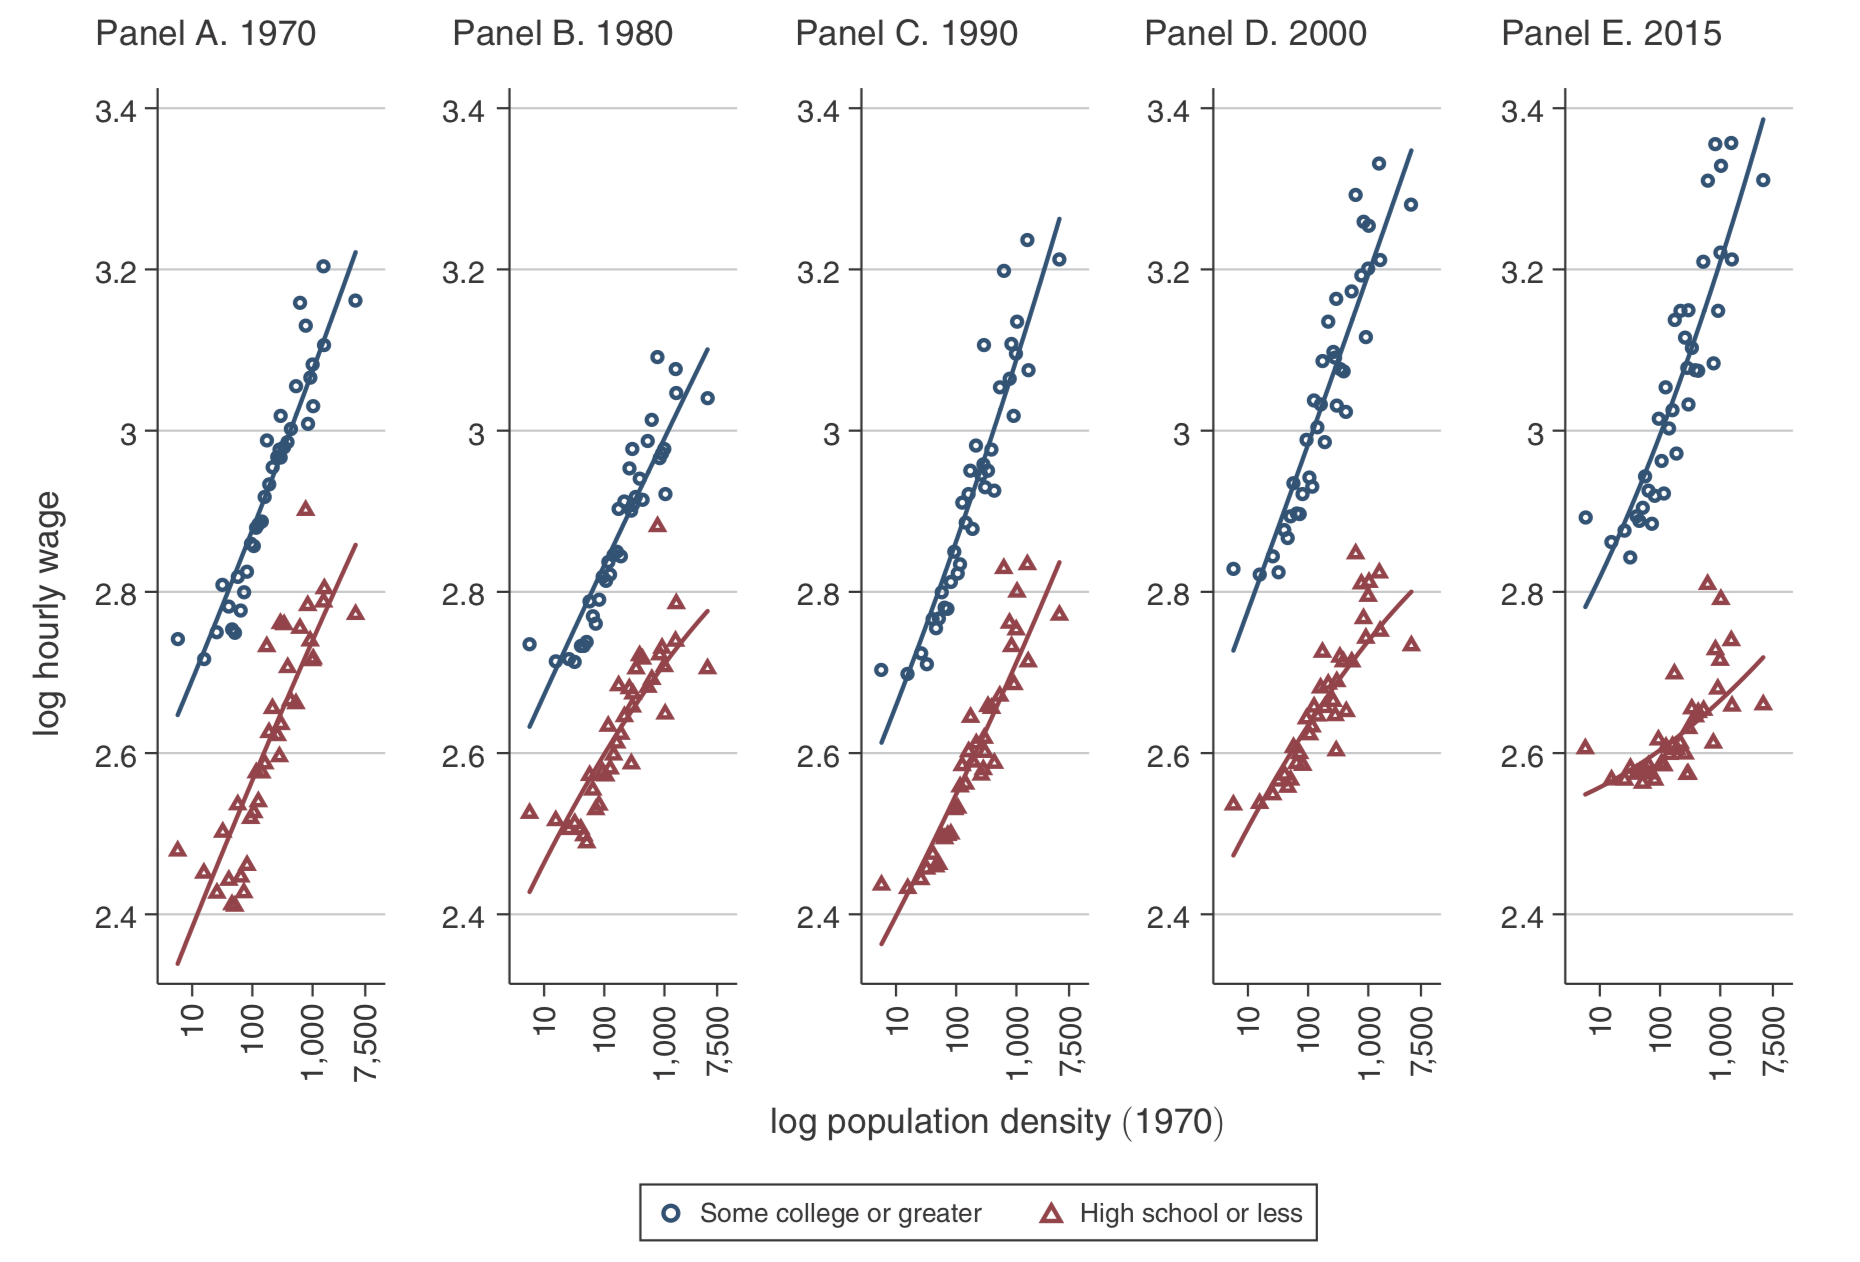
\includegraphics[scale=0.3]{Figures/Fig7_WagePremium}
		\caption{Figure plots real mean log hourly earnings among college and non-college workers in 1970, 1980, 2000, and 2015}
	\end{center}
\end{figure}

\end{frame}

\begin{frame}{Urban Wage Premium: Shifting Age Structure?}

\begin{figure}
\begin{minipage}{.5\linewidth}
	\centering
	\subfloat{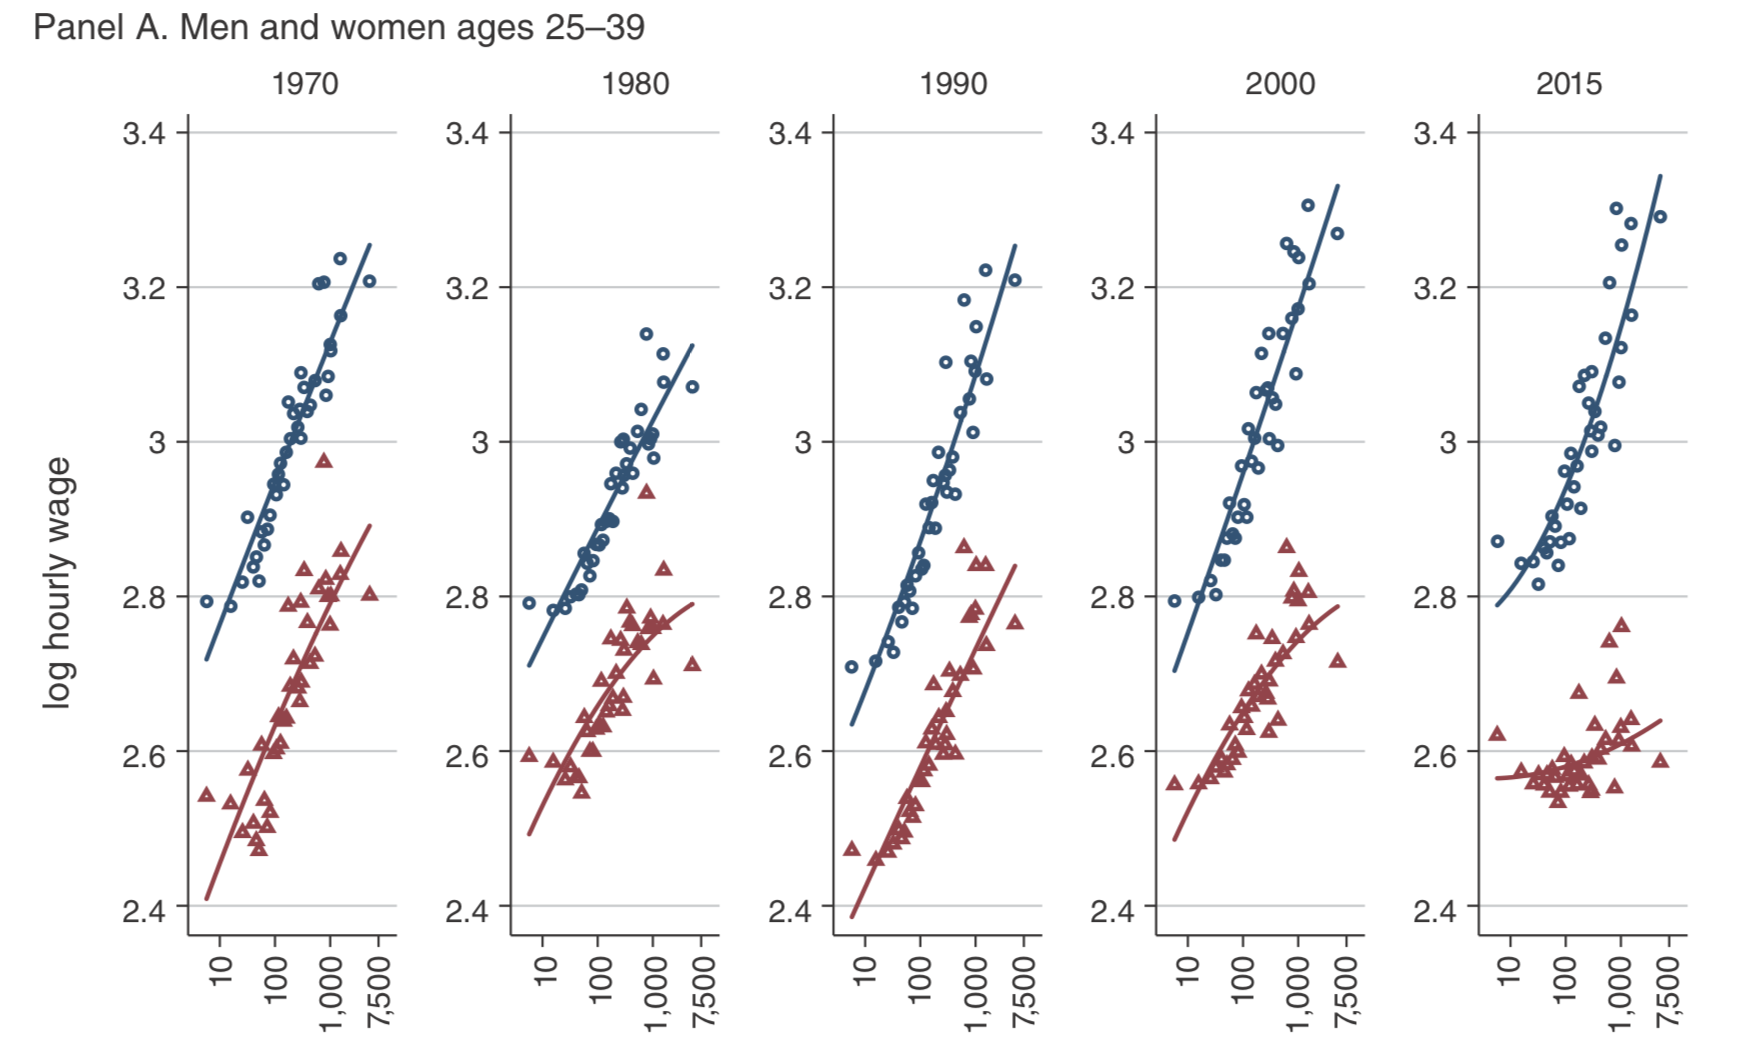
\includegraphics[scale=.17]{Figures/Fig8A_WagePremium_Age}}
\end{minipage}%
\begin{minipage}{.5\linewidth}
	\centering
	\subfloat{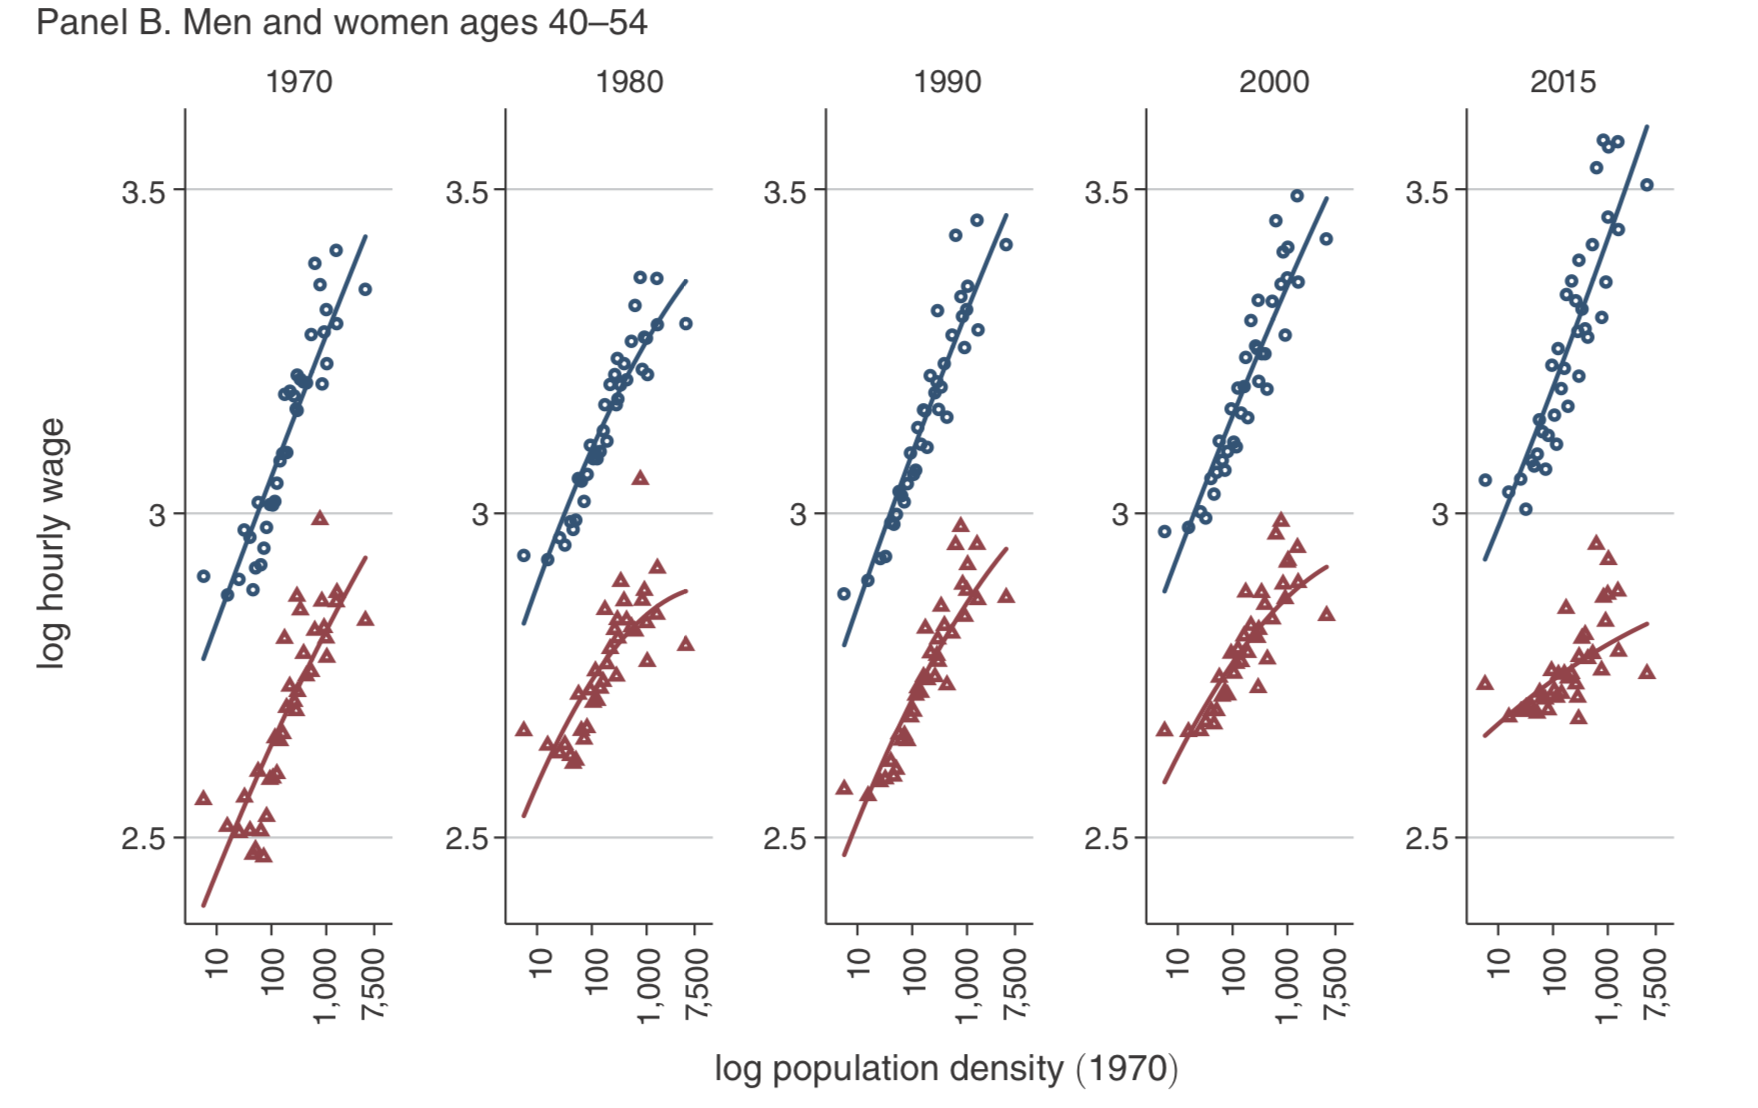
\includegraphics[scale=.17]{Figures/Fig8B_WagePremium_Age}}
\end{minipage}
\centering
\subfloat{
\includegraphics[scale=.35]{Figures/Fig8C_legend}}
	\caption{Real log Hourly Wages of College and Non-College Men and Women Ages (A) 25-39 and (B) 40-54}
\end{figure}

\end{frame}


\begin{frame}{Urban Wage Premium: Changing Education Structure and Great Recession?}

\begin{figure}
	\begin{center}
		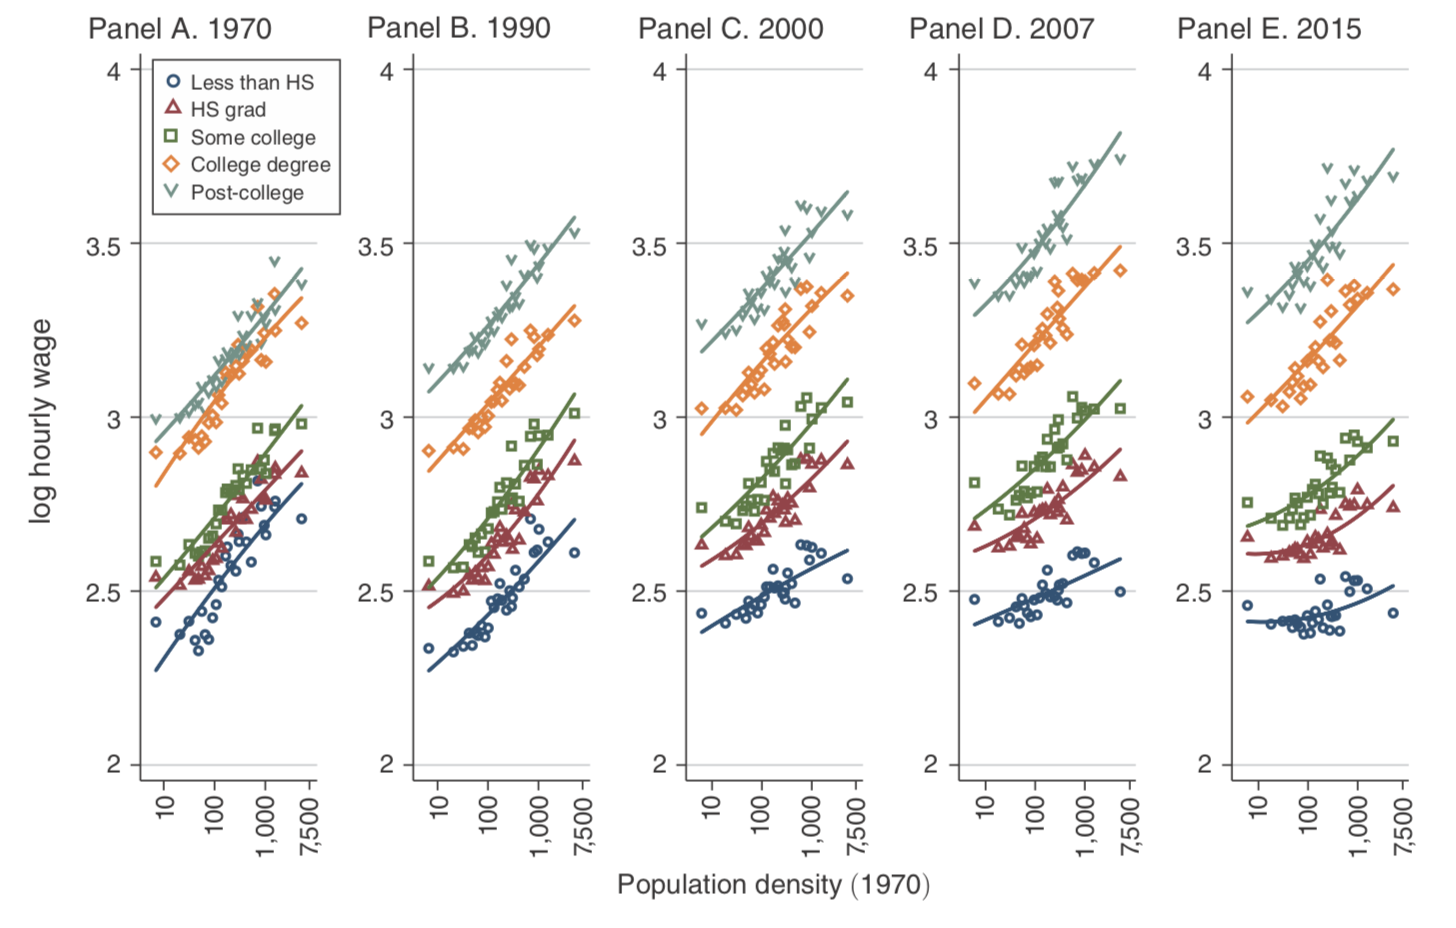
\includegraphics[scale=0.33]{Figures/Fig9_WagePremium_Education}
		\caption{Real log Hourly Wages by Detailed Education Category, 1970-2015}
	\end{center}
\end{figure}

\begin{itemize}
	\vspace{-0.7cm}
	\item Urban wage premium for non-college workers commences well before the Great Recession
	
\end{itemize}

\end{frame}

\begin{frame}{Regional Wage Divergence}

\begin{itemize}
	
	\item Figures on disappearing urban wage premium for non-college lend to regional wage divergence
	
	\bigskip
	
	\item Structural models with capital skill-complementarity and urban agglomeration conform to this
	\begin{itemize}
		\item Agglomerative forces for skilled workers have risen over time (Baum-Snow, Freedman, and Pavan, 2018).
		\item Rising agglomerative forces for skilled labor that interact positively with SBTC (Giannone, 2018).
	\end{itemize}

\end{itemize}
	
	\begin{figure}
		\begin{center}
			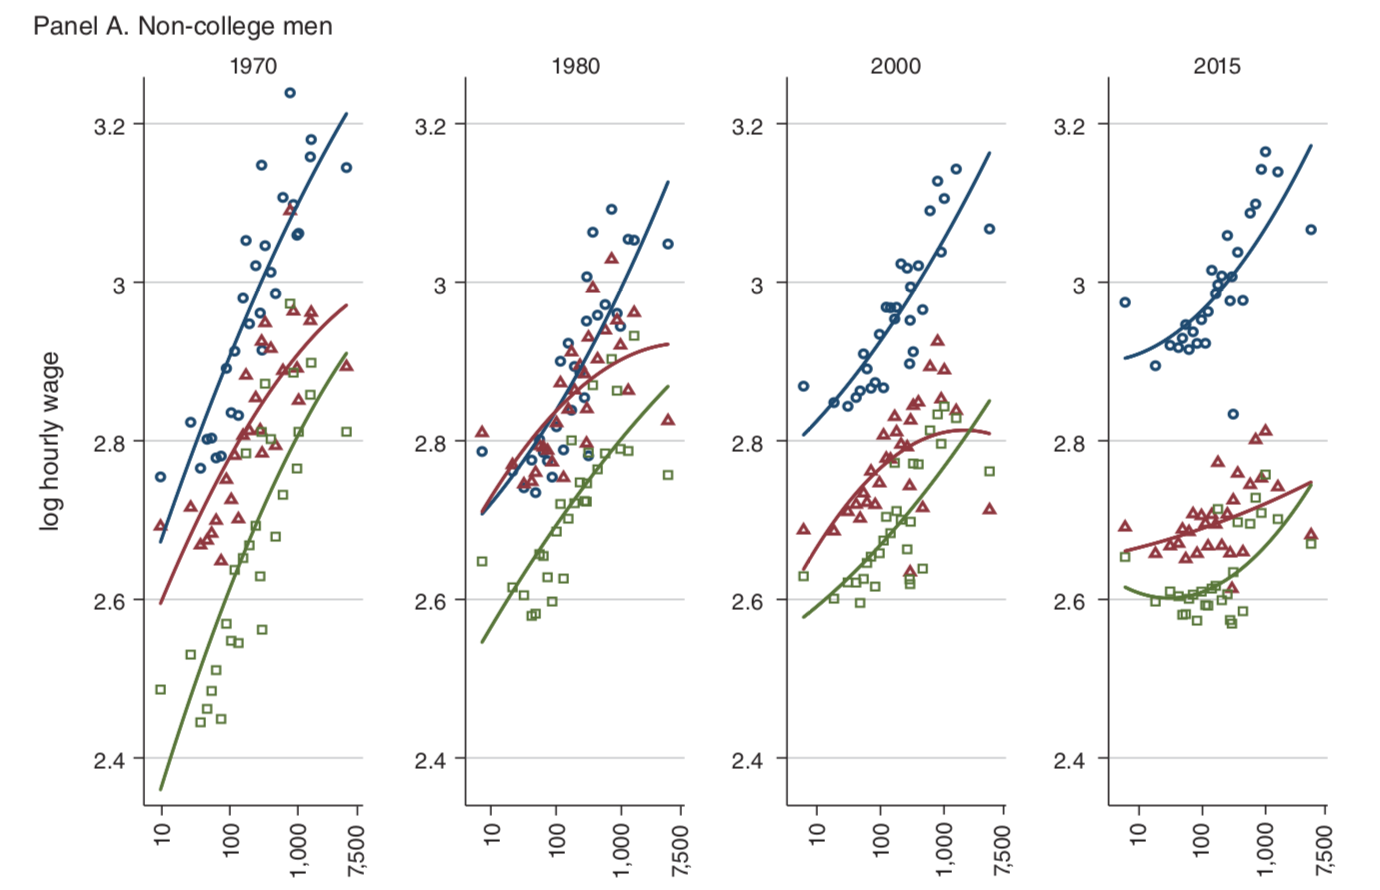
\includegraphics[scale=0.2]{Figures/Fig10_WageDivergence_Skill}
			\caption{Real log Hourly Wages by Occ. Group for non-college men, 1970-2015}
		\end{center}
	\end{figure}

%State below as comment
	%\item Patterns are consistent with falling relative demand for middle-skill work in cities.
%\begin{itemize}
	%\item However, occupation is not labor market.
	%\item Urban and non-urban wage structures are not independent via migration decisions and firm arbitrage.
%\end{itemize}

\end{frame}

\begin{frame}{Accounting for the Geography of Polarization: Wage Implications}

\begin{itemize}

	\item How would the wages of college and non-college workers have changed between 1970 and 2015 had occupational composition and occupational geography evolved as observed while wage levels by occupation and location are held fixed at their 1970 levels?
	
	\bigskip
	
	\item Going to use kernel density reweighting technique (DiNardo, Fortin, and Lemieux, 1996).
	\begin{itemize}
		\item Assumes wage change within occ. and across location. 
		\item Varies quantities while holding prices fixed.
	\end{itemize}

	\bigskip
	
	\item Estimate will be a lower bound  to the contribution of occupational change to wage changes by skill group.
	
\end{itemize}

\end{frame}

\begin{frame}{Kernel Density Reweighting}

\begin{itemize}
	
	\item Start with observed wage distribution $f(w)$. Let $\Omega_x$ be domain of covariates.
	
	\begin{equation*}
	f_{t_0}(w) = \int_{x \in \Omega_x} dF(w,x | t_{w,x} = t_0)
	\end{equation*}
	
	\item Iterating expectations: distribution of $w$ is conditioned on $x$ and the distribution of $x$ is conditioned on $t_0$,
	
	\begin{equation*}
	f_{w_{t_0}}^{x_{t_0}}(w) = \int f(w| x, t_{w} = t_0) dF(x | t_x = t_0)
	\end{equation*}
	
	\item Use identiy above to substitute in the distribution of $x$ for time $t_1$
	
\end{itemize}

\begin{align*}
f_{w_{t_0}}^{x_{t_1}}(w) &= \int f(w| x, t_{w} = t_0) dF(x | t_x = t_1) \\
&= \int f(w| x, t_{w} = t_0) \times \phi_x(x)dF(x | t_z = t_0)
\end{align*}


\end{frame}

\begin{frame}{Kernel Density Reweighting}

\begin{align*}
f_{w_{t_0}}^{x_{t_1}}(w) &= \int f(w| x, t_{w} = t_0) \times \underbrace{\phi_x(x)}_{\frac{dF(x|t_x=t_1)}{dF(x|t_x=t_0)}}dF(x | t_z = t_0)
\end{align*}

\begin{itemize}
	 
	\item $\phi_x(x)$ reweights the
	distribution of covariates in period $t_0$ to match those in $t_1$ (i.e., quantities change).
	
	\bigskip
	
	\item $f(w|x)$ held at time $t_0$ (i.e. prices are fixed).
	
	\bigskip
	
	\item Excercise will be plotting:
	\begin{enumerate}
		\item Data
		\item Reweight $f_{t_{1970}}(w)$ to reflect the changing occupational distribution during each subsequent decade
		\item (2) plus geographic component
	\end{enumerate}
	
\end{itemize}

\end{frame}


\begin{frame}{Counterfactual Wage Changes}

\begin{figure}
	\begin{center}
		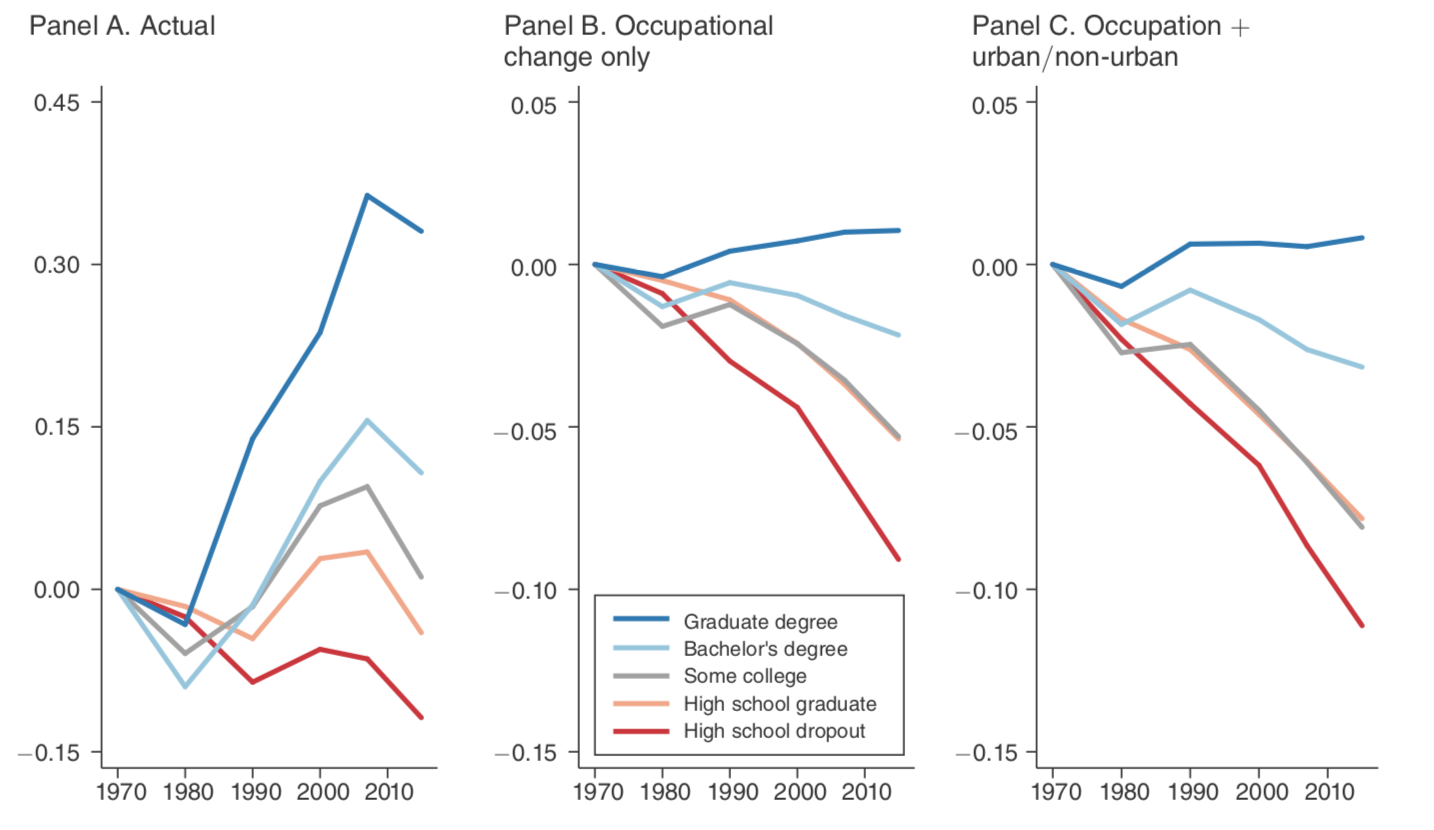
\includegraphics[scale=0.4]{Figures/Fig11_counterfactualWageChange}
		\caption{Observed and Counterfactual Changes in log Hourly Wages by Education Group, 1970-2015}
	\end{center}
\end{figure}

\end{frame}


\begin{frame}{Evaluation of Partial Equilibrium}

\begin{itemize}
	
	\item Occupational reallocation does decent job accounting for the fall in non-college wages over time interval.
	
	\bigskip
	
	\item Adding geography confirms that polarization has occurred most among urban, non-college workers.
	
	\bigskip
	
	\item Again, as earlier the partial equil. does not account for rise in college wages
	\begin{itemize}
		\item Modest occupational change for college workers
		\item Holding $w$ at 1970 level omits all productivity growth among college educated (i.e. SBTC).
	\end{itemize}

	\bigskip
	
	\item Overall cannot account for:
	\begin{itemize}
		\item Supply/demand forces on wages within and between occ.
		\item Omits increased demand for high-skill workers on college wages.
	\end{itemize}
	
\end{itemize}

\end{frame}


\begin{frame}{Where is the Land of Opportunity?}

\begin{itemize}
	

	\item What forces could restore middle-skill jobs and raise non-college wages along density gradient?

	
	\bigskip
	
	\item Firms have incentive to reinstate labor’s comparative advantage in a range of tasks (Acemoglu and Restrepo, 2018).
	
	\bigskip
	
	\item “New work” (the creation of new Census occupational titles) is concentrated in cities (Lin, 2011).
	\begin{itemize}
		\item Although, mostly held by college workers...
		\item Some "wealth work" jobs being created, e.g. yoga instructor, dog groomer, sommelier (Autor and Salomons, 2019)
	\end{itemize}

	\bigskip
	
	\item Overall, growth is in cities, but only for college workers in high-skill jobs.
	\begin{itemize}
		\item Dense cities are not alluring to low-skill occ.
		\item This is good since less migration will boost non-college wages
		\item Meanwhile, aging pop. in suburbs presents new opportunity for low-skill, labor-intensive jobs.
	\end{itemize}

	
\end{itemize}

\end{frame}


\end{document}

